\chapter{Methodology for extracting and filtering logical dependencies}
\label{extraction}

\section{Overview of the approach}
\label{sec:overview_approach}
To be done at the end


\section{Data collection}
\label{sec:data_collection}


\subsection{Data set used}
\label{subsec:data_sets_used}

\hspace{4em}To investigate logical dependencies extraction and filtering techniques and their interplay with structural dependencies, 27 open-source projects from GitHub\footnote{http://github.com/} were selected. Table \ref{table:1} provides an overview of all the software systems analyzed.

The table consists of five columns: the \textit{ID} column assigns a unique identifier to each project. The \textit{Project name} column lists the project names as they appear on GitHub. The \textit{Number of entities} column specifies the total number of entities (classes and interfaces) extracted from the source code. The \textit{Number of commits} column specifies the number of commits analyzed from the active branch (main/master) of each project. Lastly, the \textit{Type} column specifies the programming language in which the project was developed.

This selection includes projects implemented in two programming languages: Java and C\#. The systems vary in size and complexity. From a structural perspective, the smallest project is \textit{shipkit}, which contains only 639 entities, while the largest is \textit{EntityFrameworkCore}, with 50,179 entities.

Regarding commit history, \textit{shipkit} is again the smallest, with 1,563 commits analyzed, while \textit{aeron} is the largest, with 5,977 commits. This selection of projects allows a better investigation of how filtering techniques affect systems of different sizes and commit histories.


\begin{table}[!h]
\renewcommand{\arraystretch}{1}
\caption{Summary of open source projects used for logical dependencies extraction and filtering.}
\label{table:1}
\centering
\scalebox{0.9}{
\begin{tabular}{|c|c|c|c|c|c|}
\hline
   ID  & Project name   & Number of & Number of& Type\\
     &     & entites & commits & \\
\hline
1	&	bluecove	&	2685	&	894	&	Java	\\
2	&	aima-java	&	5232	&	1006	&	Java	\\
3	&	powermock	&	2801	&	949	&	Java	\\
4	&	restfb	&	3350	&	1391	&	Java	\\
5	&	rxjava	&	21097	&	4398	&	Java	\\
6	&	metro-jax-ws	&	6482	&	2927	&	Java	\\
7	&	mockito	&	5189	&	3330	&	Java	\\
8	&	grizzly	&	10687	&	3113	&	Java	\\
9	&	shipkit	&	639	&	1563	&	Java	\\
10	&	OpenClinica	&	9655	&	3276	&	Java	\\
11	&	robolectric	&	8922	&	5912	&	Java	\\
12	&	aeron	&	4159	&	5977	&	Java	\\
13	&	antlr4	&	4747	&	4431	&	Java	\\
14	&	mcidasv	&	3272	&	4136	&	Java	\\
15	&	ShareX	&	4289	&	5485	&	C\#	\\
16	&	aspnetboilerplate	&	9712	&	4323	&	C\#	\\
17	&	orleans	&	16963	&	3995	&	C\#	\\
18	&	cli	&	2063	&	4488	&	C\#	\\
19	&	cake	&	12260	&	2518	&	C\#	\\
20	&	Avalonia	&	16732	&	5264	&	C\#	\\
21	&	EntityFrameworkCore	&	50179	&	5210	&	C\#	\\
22	&	jellyfin	&	8764	&	5433	&	C\#	\\
23	&	PowerShell	&	2405	&	3250	&	C\#	\\
24	&	WeiXinMPSDK	&	7075	&	5729	&	C\#	\\
25	&	ArchiSteamFarm	&	702	&	2497	&	C\#	\\
26	&	VisualStudio	&	4869	&	5039	&	C\#	\\
27	&	CppSharp	&	17060	&	4522	&	C\#	\\
\hline
\end{tabular}
}
\end{table}




\subsection{Extracting structural dependencies}
\label{subsec:extracting_structural_dependencies}

\hspace{4em}A dependency is created between two elements that are in a relationship, indicating that one element of the relationship, in some manner, depends on the other \cite{Booch:2004:OAD:975416}, \cite{Cataldo2009SoftwareDW}.

Structural dependencies can be identified by analyzing the source code \cite{structdep}. A structural dependency between two entities (e.g., a class and an interface) exists if one entity statically depends on the other, meaning it cannot be compiled without the dependent entity. In object-oriented systems, this dependency can be given by various types of relationships: one entity extends another (for classes), implements another (for interfaces), has attributes of the other entity's type, has methods with the other entity's type in their signature, uses local variables of the other entity's type, or calls methods of the other entity \cite{Sangal:2005:UDM:1094811.1094824, CalloArias2011, 1199197}.

We use an external tool called \textit{srcML} \cite{srcML} to convert all source code files into XML files. We then extract all information about classes, interfaces, methods, or calls to other classes by parsing the XML files and building a dependency data structure. 

Maletic and Collard \cite{srcMLCollard, Collard:2011:LTF:2067850.2068011, CollardsrcML2005} developed the \textit{srcML} tool to offer an XML-based representation of the source code. The tool preserves all source code information, including comments and formatting. The tool supports languages such as C, C++, Java, and C\#, and provides command-line utilities for converting an entire project to and from the \textit{srcML} format. 

Another advantage of the \textit{srcML} tool is that it uses consistent markup for different programming languages, making it easier to extract structural dependencies from source code written in languages like Java, C++, Python, or C\#.



\subsection{Extracting Logical Dependencies}
\label{subsec:extracting_logical_dependencies}

\hspace{4em}\textit{Logical dependencies} (logical couplings) can be identified through software history analysis. Version control repositories (such as Git) store not only the source code of the system but also its change history. By examining both, we can extract structural and logical dependencies. The source code structure provides \textit{structural dependencies}, while the system’s change history reveals \textit{logical dependencies} formed by pairs of files or components that co-evolve.

As illustrated in Figure~\ref{fig:extracting_data_with_git}, the \texttt{clone} command retrieves the entire repository, including its code and commit history. The \texttt{diff} command then highlights differences between two specific commits, generating a text file that contains the differences between the two commits: code differences, the number of files changed, and the names of changed files.

\begin{figure}[H]
\centering
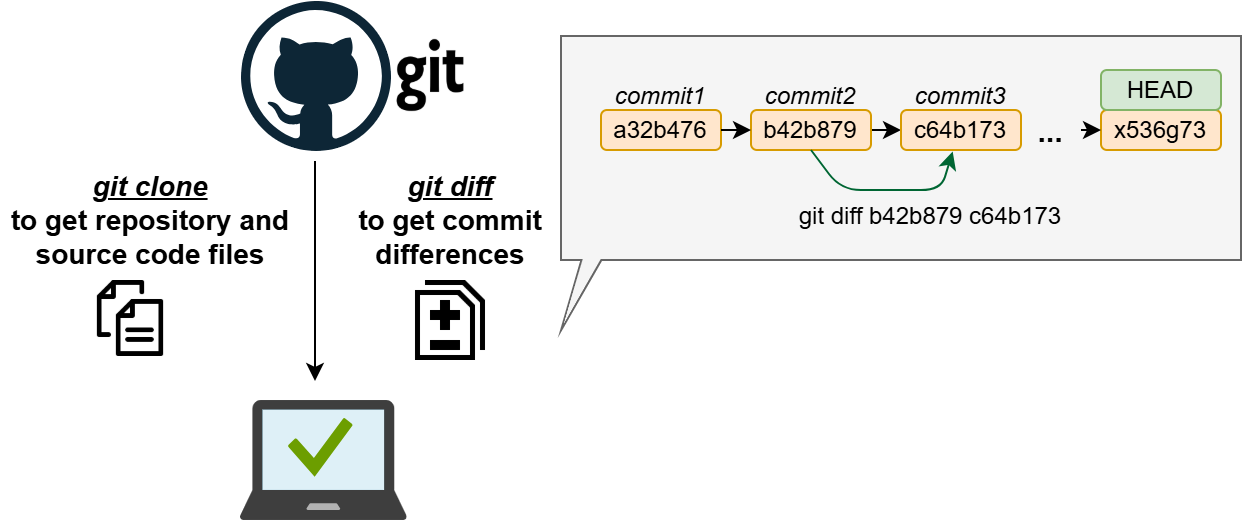
\includegraphics[width=\textwidth]{gitdata.png}
\caption{Using Git commands (\texttt{clone} and \texttt{diff}) to retrieve source code and commit changes.}
\label{fig:extracting_data_with_git}
\end{figure}


Listing \ref{lst:git_diff} provides an example of a \texttt{git diff} output for three files: \texttt{User.java}, \texttt{Calculator.java}, and \texttt{Utils.java}. From the diff output, we can identify the names of the changed files and information about added or deleted lines of code, but not the specific entities (e.g., classes or interfaces) from those files. 

To determine the changed entities, we first extract the structural dependencies of the system and create a mapping between the entities defined in each file and the file. Later, we associate the changed files with their corresponding entities when processing the diff files using this mapping \cite{DepSACI, b4, icstcc-2024, enase19}. 

For instance, in this example, the mapping can reveal that \texttt{User.java} contains the class \texttt{User}, \texttt{Calculator.java} contains the class \texttt{Calculator}, and \texttt{Utils.java} contains the class \texttt{Utils}. Even if Java typically enforces a standardized relationship between file and entity names, this is not always the case for other programming languages, so we need a uniform approach.

Using this mapping, we can say that the commit presented in Listing \ref{lst:git_diff} generates three pairs of co-changed entities: \texttt{Utils-Calculator}, \texttt{Utils-User}, and \texttt{Calculator-User}.

\begin{lstlisting}[language=diff, caption={Example output of \texttt{git diff} between two commits.}, label={lst:git_diff}]
commit 1a2b3c4d5e (HEAD -> main)
Author: Developer <developer@example.com>
Date:   Wed Dec 13 12:34:56 2024 +0000

    Refactored code and added new features.

diff --git a/src/User.java b/src/User.java
index abc1234..def5678 100644
--- a/src/User.java
+++ b/src/User.java
@@ -1,5 +1,6 @@
+    public User(String name) {
+        this.name = name;
+    }

-    public void greet() {
+    public void displayGreeting() {
         System.out.println("Hello, " + name + "!");
     }
 }

diff --git a/src/Calculator.java b/src/Calculator.java
index 9876543..2345678 100644
--- a/src/Calculator.java
+++ b/src/Calculator.java
@@ -5,7 +5,7 @@ 
-    public int subtract(int a, int b) {
+    public int subtractNumbers(int a, int b) {
         return a - b;
     }
 }

diff --git a/src/Utils.java b/src/Utils.java
index 56789ab..789abcd 100644
--- a/src/Utils.java
+++ b/src/Utils.java
@@ -3,7 +3,7 @
-    public static String getCurrentTime() {
+    public static String getFormattedTime() {
         return java.time.LocalTime.now().toString();
     }
 }
\end{lstlisting}




\section{Tool for measuring software dependencies}
\label{subsec:tool_measuring_dependencies}

To extract structural and logical dependencies, we developed a tool that takes as input the source code repository URL of a given system and extracts the corresponding software dependencies \cite{DepSACI, enase19}. 

From a workflow perspective, the tool performs three main activities: downloading the necessary data from the repository, extracting structural dependencies from the source code, and identifying and filtering co-changing pairs from the repository's commit history. Figure \ref{fig:figworkflow} illustrates these activities, with each block representing a different step from the process.


To get the source code files and the change history, we first need to know the repository URL from GitHub (GitHub is a Git repository cloud-based hosting service). With the GitHub URL and a series of Git commands, the tool can download all the necessary data for dependencies extraction.


As we can see in figure \ref{fig:extracting_data_with_git}, the \textit{"clone"} command will download a repository, including the source code files. The \textit{"diff"} command will get the differences between two existing commits in the Git repository. 
The tool gets the Git repository and the source code files by executing the "clone" command. Afterward, it gets all the existing commits within the Git repository. The commits are ordered by date, beginning with the oldest one and ending with the most recent one. The tool executes the "diff" command between each commit and its parent (the previous commit). The "diff" command generates a text file that contains the differences between the two commits: code differences, the number of files changed and changed file names.


The first step involves downloading the source code files and change history. This requires the GitHub repository URL, as GitHub is a cloud-based hosting service for Git repositories. Using this URL and Git commands, the tool downloads all the data necessary for dependency extraction.

\begin{figure}[H]
\centering
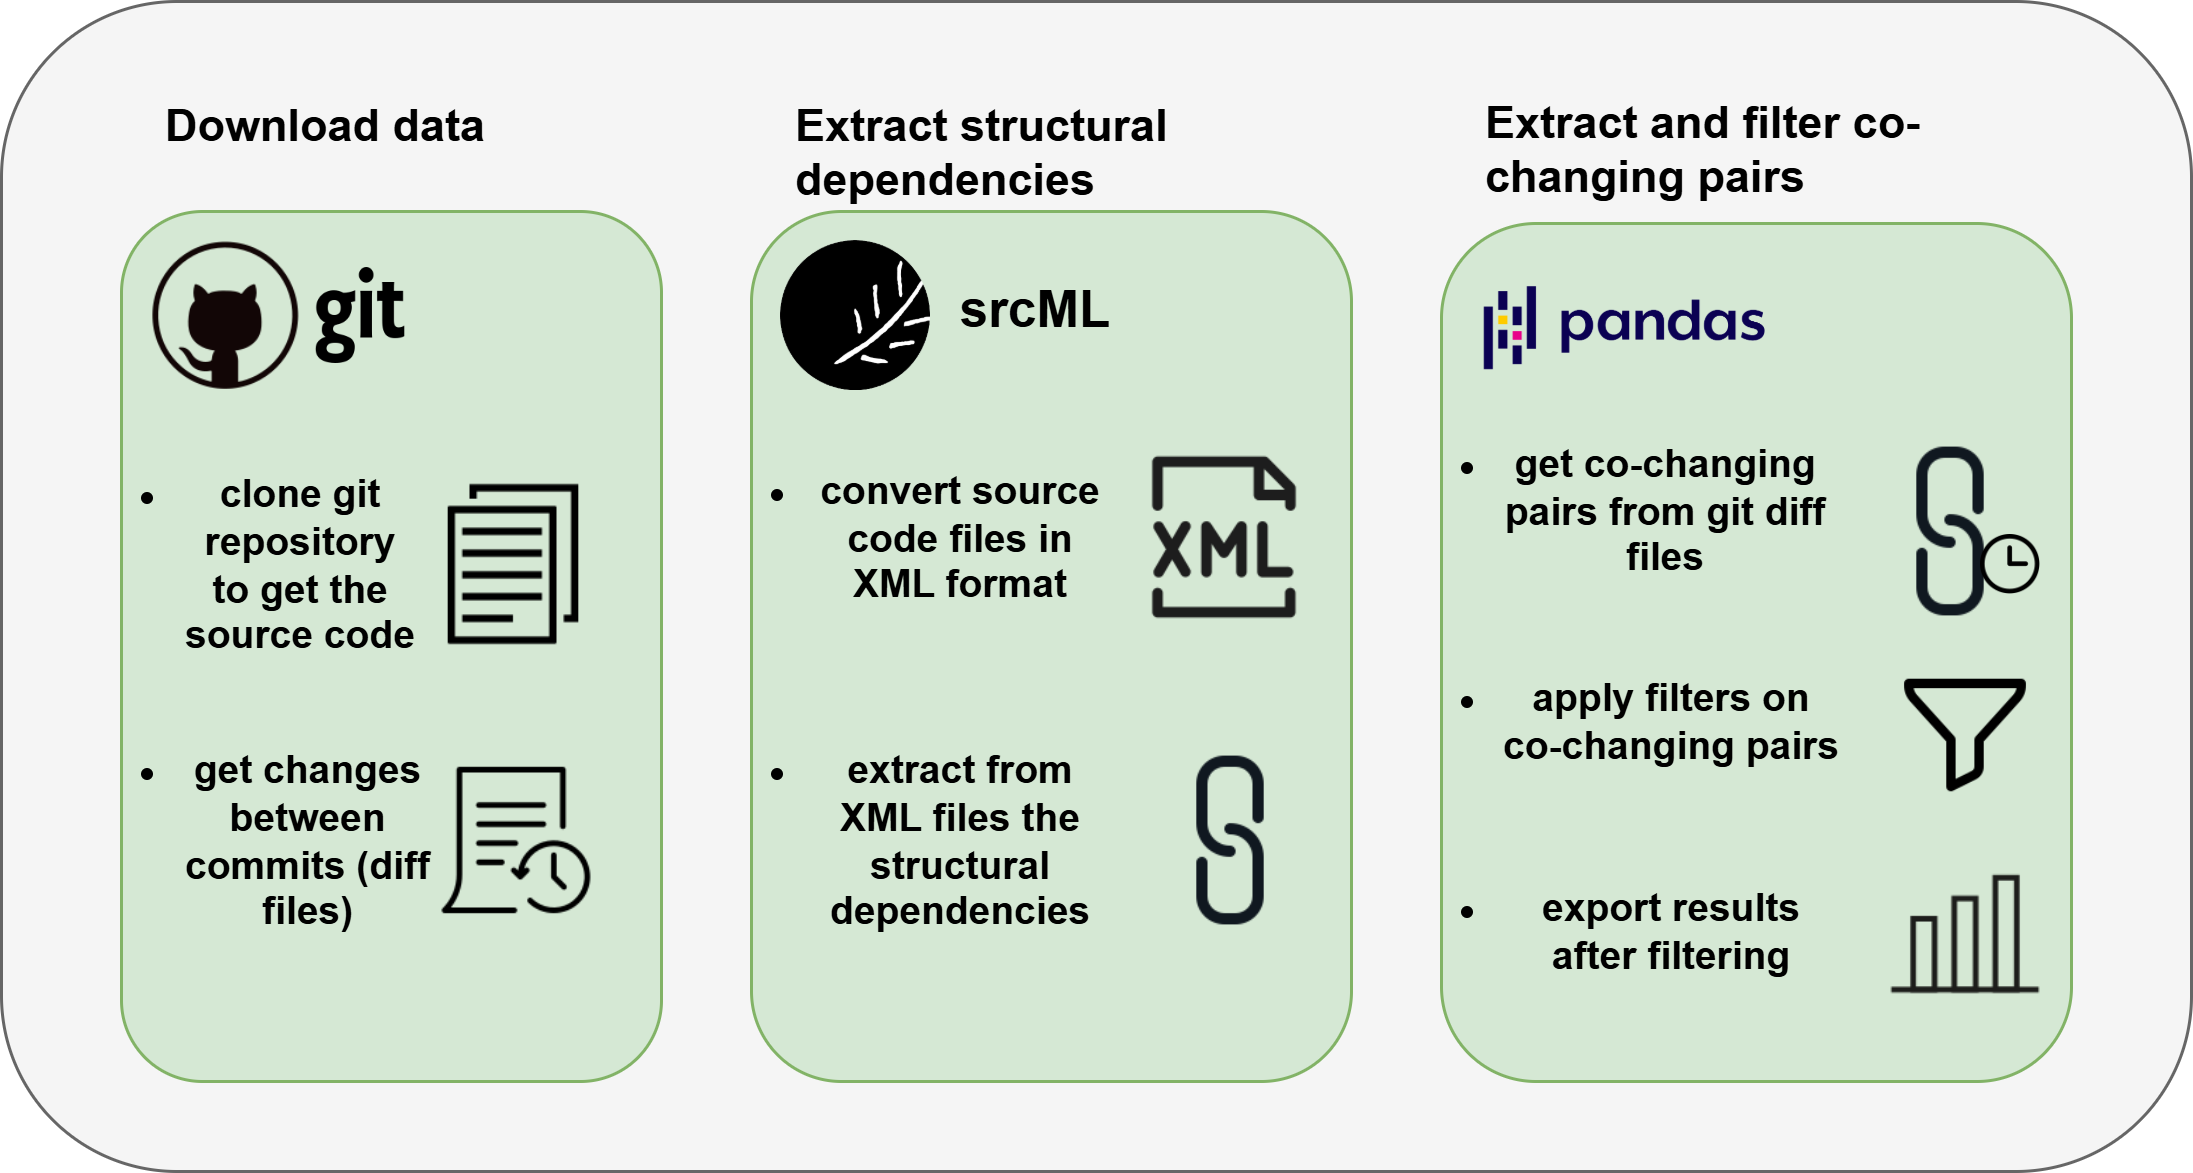
\includegraphics[width=\textwidth]{tool_workflow.png}
\caption{Tool workflow and major activities.}
\label{fig:figworkflow}
\end{figure}



\textbf{Extract structural dependencies.}

To extract structural dependencies from the source code, the tool first converts each source file into the srcML format using the method introduced in subsection \ref{subsec:extracting_structural_dependencies}. The srcML format provides an XML representation of the source code, with markup tags identifying elements of the programming language syntax\cite{srcML}. 

Once converted, the tool parses each file to identify all defined entities (such as classes, interfaces, and enums) from the file. It also detects all entities used by the defined entities. The connections between the defined and used entities form the structural dependencies.


\textbf{Extract and filter co-changing pairs.}

The process of extracting and filtering co-changing pairs is illustrated in Figure \ref{fig:figfiltering}.

To analyze the changes between commits, the tool uses the \texttt{"git diff"} command. All existing commits in the repository are collected and chronologically ordered, starting with the oldest and ending with the most recent. For each commit, the tool runs the \texttt{"git diff"} command to compare it with its parent (the preceding commit). This generates a text file containing the details of the changes between the two commits.

To extract co-changing pairs, the tool parses each generated diff file. From each file, it identifies the number of changed files and their names. Since the tool already knows the software entities contained in each file (from the structural dependencies extraction), it can determine co-changing pairs by linking entities from two different changed files. Once all the co-changing pairs for a diff file are extracted, the tool moves to the next diff file and repeats the process.

Explained in more detail in subsections \ref{subsec:filtering_transaction_size}, \ref{subsec:filtering_support}, and \ref{subsec:filtering_connection_strength}, not every extracted co-changing pair is considered a logical dependency. For a pair to be considered a logical dependency, it must pass some criteria. These criteria are implemented as filters in the tool. Each filter processes the extracted co-changing pairs and outputs the pairs that meet the configured requirements. The filters can also be combined to ensure that only meaningful logical dependencies remain after filtering.

\begin{figure}[H]
\centering
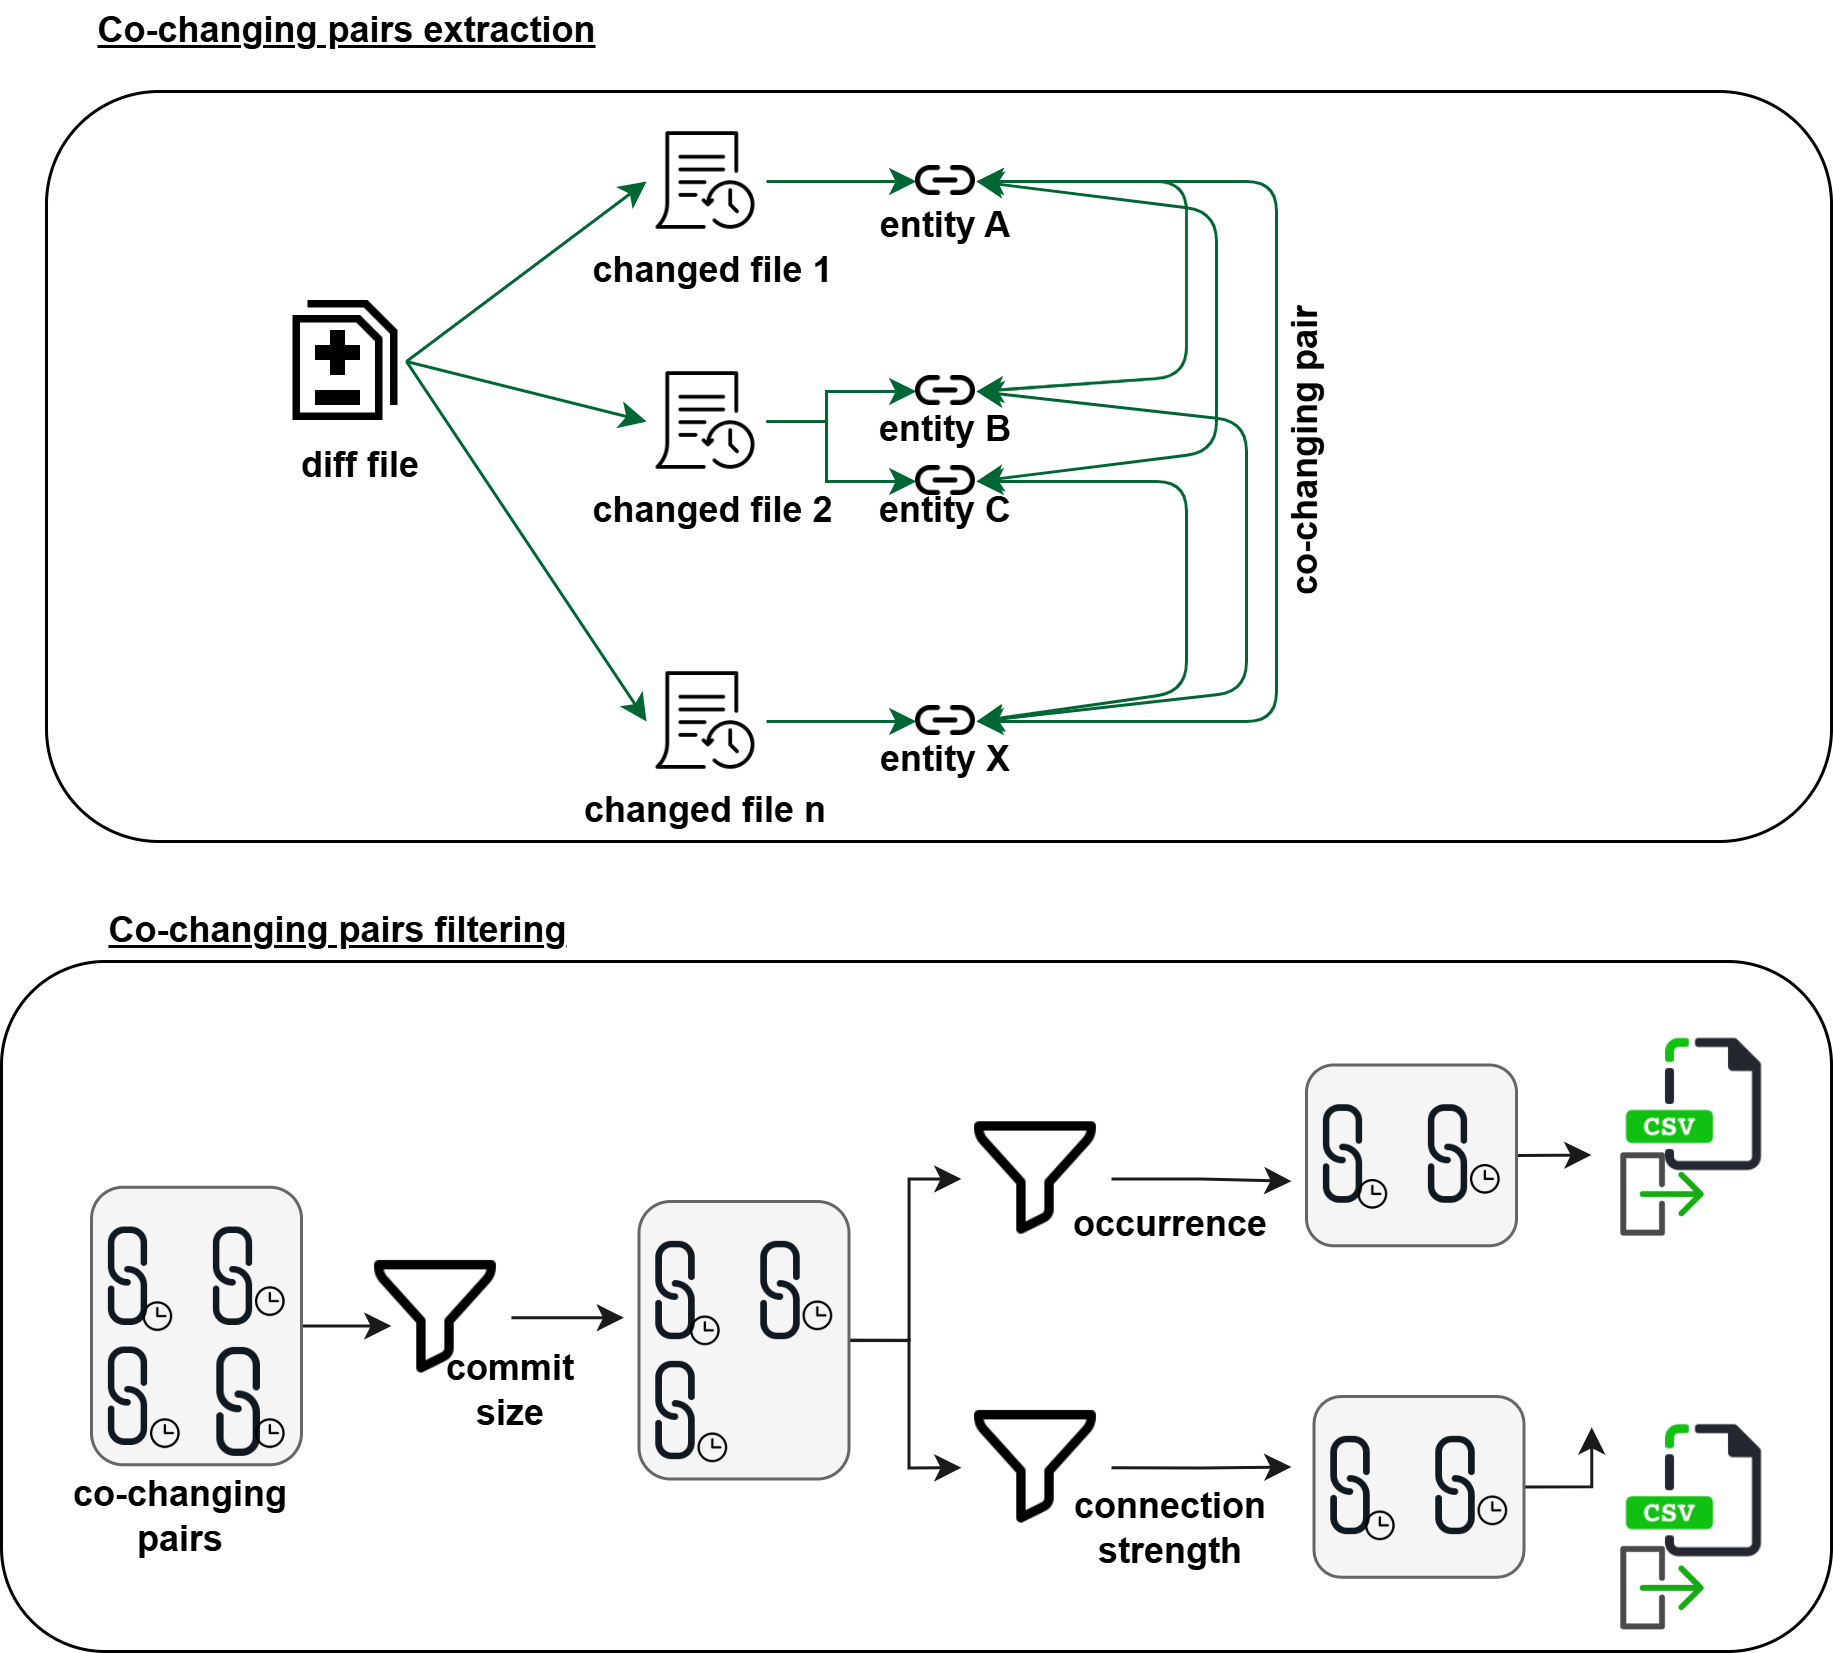
\includegraphics[width=\textwidth]{pairs_filtering.png}
\caption{Co-changing pairs extraction and filtering.}
\label{fig:figfiltering}
\end{figure}



\section{Filtering logical dependencies}
\label{sec:filtering_logical_dependencies}

\subsection{Filtering based on commit transaction size}
\label{subsec:filtering_transaction_size}

\subsection{Filtering based on support}
\label{subsec:filtering_support}


\subsection{Filtering based on connection strength}
\label{subsec:filtering_connection_strength}

